\documentclass[12pt]{article}
\usepackage{parskip}
\usepackage{amsmath}
\usepackage{pdfpages}
\usepackage{listings}
\usepackage{color}
\usepackage[margin=.6in]{geometry}

\definecolor{dkgreen}{rgb}{0,0.6,0}
\definecolor{gray}{rgb}{0.5,0.5,0.5}
\definecolor{mauve}{rgb}{0.58,0,0.82}

\lstset{frame=tb,
  language=C++,
  aboveskip=3mm,
  belowskip=3mm,
  showstringspaces=false,
  columns=flexible,
  basicstyle={\small\ttfamily},
  numbers=none,
  numberstyle=\tiny\color{gray},
  keywordstyle=\color{blue},
  commentstyle=\color{dkgreen},
  stringstyle=\color{mauve},
  breaklines=true,
  breakatwhitespace=true,
  tabsize=3
}
\begin{document}

\includepdf[pages={2}]{02.pdf}
\includepdf[pages={3}]{02.pdf}
\includepdf[pages={4}]{02.pdf}

\includepdf[pages={6}]{02.pdf}
\includepdf[pages={7}]{02.pdf}

Most micro-controllers contain general purpose registers that take the role of the MAR and the MBR. On the CPU we have some registers but they result in a very small amount of memory (8-64 bits in size). Those registers are connected to main memory (0x0000-0xFFFF). Bits of this memory is mapped to flash and RAM and other bits of memory. For each chunk of memory we take a small piece where we store useful functions that allow processor to interact with main memory.

\includepdf[pages={8}]{02.pdf}
\includepdf[pages={9}]{02.pdf}
In most computer architectures the program lives in RAM or micro-controllers. The program counter always contains the address of the next instruction for the program.

\includepdf[pages={10}]{02.pdf}
You can use the voltile keyword or a cobbler list to keep the computer from optimizing certain registers.

\includepdf[pages={11}]{02.pdf}
\includepdf[pages={12}]{02.pdf}
We want to hide control and status registers from the user but still have them around to show the status that the computer is in.

\includepdf[pages={13}]{02.pdf}

\includepdf[pages={14}]{02.pdf}
Brownout and watchdog are flags that talk about the powerstate of the system and allows for an interrupt based on it

\includepdf[pages={15}]{02.pdf}
\includepdf[pages={16}]{02.pdf}

\includepdf[pages={18}]{02.pdf}
\includepdf[pages={19}]{02.pdf}
\includepdf[pages={20}]{02.pdf}
A thing to keep in mind is that the PC points to the next instruction after the fetch stage, this can fuck shit up if you use it incorrectly.

\includepdf[pages={21}]{02.pdf}
\includepdf[pages={22}]{02.pdf}

Operation 1 is a load operation into a accumunlator, operation 2 is a store that to memory, and operation 3 is a add to that from memory.

\includepdf[pages={23}]{02.pdf}
In the initial condition we have the PC pointing to the next isntruction after the fetch (300). So the instruction that we have is number 1 (the load operation). During the execution we go to the address and get the data there and  incrememnt the PC. In 301 we have the store command which we enact. Etc for the other command. We call this a two stage pipeline.

\includepdf[pages={25}]{02.pdf}
Since most peripherals are slower than the computer so we use interrupts to make the program go at their stage, then return to the compture. To do this we need to change the execution cycle.

\includepdf[pages={26}]{02.pdf}
\includepdf[pages={27}]{02.pdf}
In a program that doesnt have interrupts. We have a linear program that exectues, like the example before. When we need to interact with an IO device (say to read or write) so we need to do a subroutine call which involves spinning up some hardware (say a hard drive) so we are limited by the speed at which that call can be made (suuuper slow).

\includepdf[pages={28}]{02.pdf}

 We isolate the waiting portion allowing us to go back to the main program while we wait for the IO. The write operation only executes the set up part and immediatly returns to the program and exectures the rest of the program. When the IO is done with its shit it interrupts the program to call it to finish the execution of that call now that the data needed is there. Then the program finishes doing its thing.

 \includepdf[pages={29}]{02.pdf}

We can run into problems when we have multiple calls to the IO in a short period of time which means that we need to wait for the first call to finish before the second one can go. You can't really make a queue at the IO of commands, so the program grids to a halt.

Need to check the disk status before attempting to read or write.

\includepdf[pages={30}]{02.pdf}
When an interrupt happens we need to store a snapshot of the program so that we can return to the same state once the interrupt handler is done.

\includepdf[pages={31}]{02.pdf}
The interrupt handler should save all the state of the program and then return that state once its done dealing with its shit. It also needs to reset the program status word and the pc value. The program status word contains the flags from the operation and a whole bunch of shit it didnt get since he talks to quickly. Basically this guy is really important to restore.

\includepdf[pages={35}]{02.pdf}
The first thing that happens, before the interrupt handler, is pushing the PSW onto the stack (remember stack pushes downward in memory). Next we push on the program counter, counts as the state of the program since this is just a pointer to it. Now we can enact the interrupt service routine. A interrupt vector is a table numbering all of th interrupts within which are the starting addresses of each of the interrupt service routines that service it. To start the interrupt handler make the PC equal to that address. We cannot start that yet though since there is still a ton of data unsaved (local variables and such).  The hardware used in this course does some of this for us in the exception stack register (not fully sure on the name). Once this is pushed onto the stack we can safely start the interrupt handler.

Once the interrupt service routine we write all of the general registers used by the program off of the execution stack in reverse order. Return from interrupt (RTI) on ARM restores the PC and PSW for us.

If you have any stateful libraries (things that need to know what happened to the past) you need to store their state onto the stack so that they dont lose their place in the interrupt. Basically if you use the memory, you need to store it (store all data registers).

%checkout the ARM TRM manual for details on hos the RTI works GCC manual for something I couldn't read

\includepdf[pages={36}]{02.pdf}
\includepdf[pages={37}]{02.pdf}

When an interrupt occurs, store a snapshot by saving the necessary registers. When you return from it make sure you pop in reverse order

\includepdf[pages={38}]{02.pdf}

When you have multiple interrupts the interrupt vector already prioritizes interrupts so when multiple interrupts occur you can make sure that the top one is executed or you can have nested interrupts that each defer things as they go to the next highest in the list. I think

%review this.

\includepdf[pages={35}]{02.pdf}
This page is very important to know for the exam. Hardware support ends after the PC is moved to point at the interrupt handler. The software needs to handle the saving and restoring of data and PC/PSW when its done.

\begin{lstlisting}
    void UART_ISR() {
        prologue //save all data and necissary registers (push R0 ... R15)
        ...
        compiled c compiled
        ...
        epilogue //reload all data and registers (pop R15 ... R0)
        RTI
    }
\end{lstlisting}

Modern computer architectures don't really care about assembly and assume you use c programming. This means that the hardware will do alot of the saving of registers for us.

\begin{enumerate}
    \item hardware pushes R0..R4, R13, R14 (called exception stack frame)
    \begin{enumerate}
        \item R15 = PC
        \item R14 = Link Register
        \item R13 = Stack Pointer
    \end{enumerate}
    \item writes a special value in the link register to 0xffff
    \item execute interrupt service routine (the steps below are baked onto the board)
    \begin{enumerate}
        \item prologue of ISR (pushing of registers) is usually a c function, described in standard for ARM
        \item store R4-R12
        \item exectute handler
        \item store the result of the funtion in R0
        \item pop R4-R12
        \item return to code (BX LR)
    \end{enumerate}
\end{enumerate}

\includepdf[pages={39}]{02.pdf}
\includepdf[pages={40}]{02.pdf}
\includepdf[pages={41}]{02.pdf}
\includepdf[pages={42}]{02.pdf}
\includepdf[pages={43}]{02.pdf}
\includepdf[pages={44}]{02.pdf}

\begin{enumerate}
    \item Start IO read command
    \item Return to program
    \item program is interrupted when the IO read is done and ready to be used
\end{enumerate}

\includepdf[pages={45}]{02.pdf}


\includepdf[pages={47}]{02.pdf}
\includepdf[pages={48}]{02.pdf}
\includepdf[pages={49}]{02.pdf}
We want to organize the access that we need to make to be as little as possible (use fast memory whenever possible) by abusing the fact that memory acesses by the user ten to cluster, so when we access slooooooow memory we want to return a lot of data so that we dont have to access it as often.
\includepdf[pages={50}]{02.pdf}


\end{document}
